\chapter{Related Work}
\label{ch:related_work}
This chapter describes the research presented in this thesis in the
context of similar work, with particular emphasis on the simulation
methodology used.  For a similar review with greater detail on the
simulation results and the conclusions that have been drawn from them, the
interested readers is referred to \cite{weidlich:08}.

In the interests of repeatability, the software developed for this thesis has
been released as open source under a project named Pylon.  The end of this
chapter describes the software project in the context of other open source
electric power Engineering tools and explains the contribution that has
been made.

\section{Custom Learning Methods}
Early agent-based electricity market simulations in the literature do not
utilise traditional learning methods from Artificial Intelligence, but rely
upon custom heuristic methods.  They are typically formulated using the
author's intuition and encapsulate basic trading rules, but disregard many of
the key concepts from reinforcement learning theory.

\subsection{Market Power}
Under Professor Derek Bunn, researchers from the London Business School
performed some the first and most reputable agent-based electricity
market simulations in the literature.  Their research was initially motivated
by proposals in 1999 to transform the structure of The England and Wales
Electricity Pool with the aim of combating generator market power, that was
widely believed to be causing elevated market prices.

In \cite{bower:2001} a
detailed model of electricity trading in England and Wales is used to compare
day-ahead and bilateral contract markets under uniform price and
discriminatory settlement.  Twenty generating companies operating in the Pool
during 1998 are modelled as agents endowed with a portfolio of generating
plants.  Plant capacities, costs and expected availabilities are synthesised
from public and private data sources and the author's own estimates.  In
simulations of the day-ahead market, each agent submits a single price for the
following simulated trading day, for each item of plant in its portfolio.
Whereas, under the bilateral contract model, 24 bids are submitted for each
generator, cooresponding to each hour of the following simulated day.  Revenues
are calculated at the end of each trading day and are determined either by the
bid price of the marginal unit or the generator's own bid price.  Each
generating plant is characterised in part by an estimated target utilisation
rate that represents its desire for forward contract cover.  The agents learn
to achieve this utilisation rate and then improve profitability.

Algorithm X defines the rules followed by each agent.  If the
utilisation rate is not achieved, a random percentage from a uniform distribution with a
range of $\pm10\%$ and $0\%$ mean is substracted from the bid price of all
generators in the agent's portfolio.  Agents with more than one generator
transfer successful bidding strategies between items of plant by setting the
bid price for a generator to the level of the next highest submitted bid price if
the generator sold at a price lower than that of other generators in the same
portfolio.  If an agent's total profit does not increase, a random percentage
from the same distribution as above is added or subtracted from the bid price
from the previous day for each of its generators.  A cap on bid prices is
imposed at \pounds1000 in each period.  Demand follows a 24-hour profile based
on the 1997/98 peak winter load pattern.  The response of the load schedule to high prices is
modelled as a reduction of 25MW for every \pounds1/MWh that the system marginal
price rises above \pounds75/MWh.

750 trading days are simulated for each of the four combinations of a day-ahead
market and the bilateral model under uniform pricing and discriminatory
settlement.  Prices are found to generally be higher under pay-as-bid pricing
for both market models.  Agents with larger portfolios are shown to have a
significant advantage over smaller generators due to their greater ability to
gather scarce market price information and distribute it among generators.

In \cite{bower:2001b} a more sophisticated custom learning method, resembling
the Roth-Erev method described in Appendix \ref{sec:rotherev}, is applied to a
more detailed model of the New Electrcity Trading Arragements.  The balancing mechanism is modelled as a one-shot
market, that follows the contract market, to which increment and decrement
bids are submitted.  Active demand side participation is modelled
and generator dynamic constraints are represented by limiting the number of off/on
cycles per day, but again, transmission constraints and regional variations
are ignored.

Supplier and generator agents are assigned an optimal value for
exposure to the balancing mechanism that is typically low due to high price and
volume uncertainty.  The agents learn to maximise profit, but profits are
penalised if the objective for balancing mechanism exposure is not
achieved.  They learn policies for pricing markups on the bids submitted
to the power exchange and the increments and decrements submitted to the
balancing mechanism.  Markups in the power exchange are relative to to prices
from the previous day and markups on balancing mechanism bids are relative to
power exchange bid prices on the same day.  Different markup
ranges are specified for generators and suppliers in the power exchange and
balancing mechanism and each is partitioned into ten discrete intervals.

As with the Roth-Erev method, a probability for the selection of each markup is
calculated by the learning method.  Daily profits and acceptance rates for
bids/offers from previous trading days are extrapolated out to determine
expected values and thus the expected reward for each markup.  The markups are then
sorted by expected reward in decending order.  The perceived utility of each
markup $j$ is
\begin{equation}
U_j = \mu \biggl(\frac{\phi - n}{\phi}\biggr)^{i_j-1}
\end{equation}
where $i$ is the index of $j$ in the ordered vector of markups and $\phi$ is a
search parameter.  High values of $\phi$ cause the agent to adopt a more
exploratory markup selection policy.  For all of the experiments $\mu = 1000$,
$\phi = 4$, $n = 3$ and the probability of selecting markup $j$ is
\begin{equation}
Pr_j = \frac{U_j}{\sum_{k=1}^K U_k}
\end{equation}
for $K$ possible markups.

A representative model of the England and Wales system with 24 generator
agents, associated with a total of 80 generating plants, and 13 supplier agents
is analysed over 200 simulated trading days.  The authors draw conclusions on
the importance accurate forecasts, greater risk for suppliers than generators, the
value of flexible plant and the influence of capacity margin on opportunities
for collusive behaviour.

The same learning method is applied in \cite{bunn:03} as part of an
inquiry by the Competition Commision into whether two specific companies in the
England and Wales electricity market had enough market power to operate against
the public interest.

Another early publication on agent-based simulation of electricity markets in
which a custom learning method is used is \cite{visud:99}.  The simulations
comprise only three generators, market power is assumed, and the authors
analyse the mechanisms by which the market power is exercised.  Two bid formats
are modelled.  The \textit{single-step supply function} model requires each
generator to submit and price and a quantity, where the quantity is determined
by the generator's marginal cost function.  The \textit{linear supply
function} model requires each generator to submit and value corresponding to
the slope of its supply function.  The bid price or slope value for generator
$i$ after simulation period $t$ is
\begin{equation}
x_i(t+1) = x_i(t) + b_i(p_m(t))u_i(t)
\end{equation}
where $b_i \in \lbrace-1,0,1\rbrace$ is the reward as a function of the market
clearing price $p_m$ from stage $t$ and $u_i$ is a reward gain or attenuation
parameter.  The reward $b_i$ is defined according to strategies for estimated
profit maximistaion and competition to be the base load generator.  Both
elastic and inelastic load models are considered.  Using the single-step supply
function model, the two strategies are compared in a day-ahead market setting,
using a case where there is sufficient capacity to meet demand and a case where
there is excessive capacity to the point where demand can be met by just two of
the generators.  The linear suuply model is analysed using moth day-ahead and
hour-ahead markets with inelastic load.  The hour-ahead simulation is repeated
with elastic demand response.

The first coauthor goes on to compare a similar custom learning method with two
other algoithms in her thesis \cite{visud:thesis}.  The custom method is
designed specifically for the power pool model that is implemented and uses
separate policies for selecting bid quantities and prices according to a slew of if-then
rules that attempt to capture capacity withholding behaviour.  The method is
compared with algorithms developed in \cite{auer:03} for application to the
$n$-armed bandit problem \cite[\S2.1]{robbins:53,suttonbarto:1998} and a method
based on evaluative feedback with softmax action selection
\cite[\S2]{suttonbarto:1998}.

In the algorithms from \cite{auer:03} each action $i = 1,2,\dotsc K$ for $K$
possible actions is associated with a weight $w_t(i)$ in simulation period $t
\in T$, where $T$ is the total number of simulation periods, that is used in
determining the action's probability of selection
\begin{equation}
p_i(t) = (1 - \gamma) \frac{w_i(t)}{\sum_{j=1}^K w_j(t)} + \frac{\gamma}{K}
\end{equation}
where $\gamma$ is a tuning parameter, with $0 < \gamma \leq 1$, that is
initialised such that
\begin{equation}
\gamma = \min \Biggl\lbrace \frac{3}{5}, 2\sqrt{\frac{3}{5} \frac{K\ln K}{T}}
\Biggr\rbrace .
\end{equation}
Using the received reward $x_t(i_t)$, the weight for action $j$ in period
$t+1$ is
\begin{equation}
w_{t+1}(j) = w_t(i) \exp \biggl(\frac{\gamma}{3K} \biggl(\hat{x}_t(i) +
\frac{\alpha}{p_t(i)\sqrt{KT}}\biggr)\biggr)
\end{equation}
where
\begin{equation}
\hat{x}_t(i) =
\begin{cases}
x_t(j)/p_t(i)& \text{if $j=i_t$}\\
0& \text{otherwise}
\end{cases}\end{equation}
and
\begin{equation}
\alpha = 2\sqrt{\ln(KT/\gamma)}.
\end{equation}

In the evaluative feedback method from \cite[\S2]{suttonbarto:1998} each action
$i$ has a value $Q_t(i)$ in simulation period $t$ equal to the expected average
reward if that action is selected.  The softmax method uses a Boltzman
distribution to select actions with probability
\begin{equation}
p_t(i) = \frac{e^{Q_t(i)/\tau}}{\sum_{j=1}^K e^{Q_t(j)/\tau}}
\end{equation}
where $\tau$ is a \textit{temperature} parameter with $\tau > 0$.  The value of
action $i$ in the $(t+1)^{th}$ period is
\begin{equation}
Q_{t+1}(i) = \begin{cases}
(1-\alpha)Q_t(i) + \alpha r_t(i) & \text{if $i_{t+1}=i$}\\
Q_t(i) & \text{otherwise}
\end{cases}
\end{equation}
where $\alpha$ is a constant \textit{step-size} parameter with $0 < \alpha
\leq 1$.

An extensive suite of simulation reuslts are reported and the choice of
learning method is found to have a significant impact on agent performance, but
no quantitative comparison measure is provided and no conclusions as to which
method is the superior are drawn.

\subsection{Financial Transmission Rights}
In \cite{ernst:04} a custom learning method is defined and used to study
generator and supplier profits where financial transmission rights are part of
the market.  A two node transmission system is defined with one lossless
transmission line of limited capacity, endowed to a transmission operator
agent.  Generator agents submit bids for their respective generating plants
and the transmission owner submits a bid representing the cost per MW of
transmitting power between the nodes.  The market operator clears the bids,
minimising costs while balancing supply and demand and not violating the line
capacity.  Prices at each node are calculated to provide a signal for both
energy and transmission costs.

Each agent selects its bid according to a
calculation of the reward it would expect to receive if all other agents were
to bid as they did in the previous stage.  If multiple bids are found to have
the same value then the least expensive is selected.  In the first period,
previous bids are assumed to be at marginal cost.  Several case studies are
examined with different numbers of generators and line capacities, but few
concrete conclusions are drawn.

% \section{Agent-Based Simulation}
% Relative to the traditional closed-form equilibrium approaches, agent-based
% simulation of (electricity) markets is a new field of research.  For
% comprehensive reviews and surveys of the many different techniques that have
% been applied in recent years the interested reader is directed to
% \cite{weidlich:08,tesfatsi:handbook,visud:thesis}.  This section will focus on
% reviewing literature from the field in which reinforcement learning techniques
% were applied in combination with explicit power system models.  A short review
% is also provided of some more general applications of reinforcement learning
% with connectionist systems and policy-gradient methods.

% Game theoretic models are commonly associated with economics and attempt to
% capture behaviour in strategic situations mathematically.  They have been
% applied to electric energy problems of many forms, including but not limited
% to analysis of market structure, market liquidity, pricing methodologies,
% regulatory structure, plant positioning and network congestion.  More
% recently, agent-based simulation has received a certain degree of attention
% from researchers and has been applied in some of these fields also.
%
% While popular and seemingly promising, agent-based simulation is still centred
% around abstracted models.  The assumptions made is this abstraction must be
% subjected to the same verification and validation as with equation-based
% models.  Verification of assumptions and model validation are often overlooked
% in agent-based simulations of energy markets, yet they are possibly the most
% important steps in the model building process.  Techniques used to develop,
% debug and maintain large computer programs can often be used to verify that a
% model does what it is intended to do.
%
% Validation of an energy market model is more difficult.  It can be accomplished
% using the intuition of experts or through comparison of simulation results
% with either historical market data or theoretical results from more abstract
% representations of the model.  Finding verifyable trends in existing markets
% is a very large challenge.  To then prove that a computational model
% replicates these characteristics with suitable fidelity is yet more
% challenging still.  Only when a model is suitably verified and validated can
% any conclusions be drawn from results obtained through implementation and
% simulation of suitable scenarios.

\section{Simulations Applying Q-learning}
% Krause et al.\ have published agent-based energy market research in which
% Q-learning methods were applied while considering physical system properties.
% In a comparison between Nash equilibrium analysis and agent-based simulation,
% the suitability of bottom-up modelling for the assessment of market evolution
% was assessed\cite{krause:nash}.  This is built upon in subsequent publications
% which evaluate the influence on market power and social welfare of three
% congestion management schemes and which analyse strategic behavior in combined
% gas and electricity markets\cite{krause:cong,krause:gas}.  Power Transmission
% Distribution Factors (PTDF) are used in place of explicit power flow equations
% in determining line flows.  The action domain of generating agents is limited
% to 0\%, 5\% and 10\% markups on true marginal costs.  The implementation of the
% Q-learning method used does not differentiate between environment states when
% selecting actions. This is a modification to the traditional formulation that
% still results in convincing conclusions, as with the popular Roth-Erev method.
%
% There are similar applications of Q-learning in which states \textit{are}
% defined, but none model the AC transmission system.  A common approach is to
% use categorised market price from the previous period as state
% information\cite{bakirtzis:psce,xiong:discrim}.
Agent-based simulation of electricity markets has been carried out with
participants behavioral aspects modelled using the Q-learning methods
described in Appendix \ref{sec:qlearning}.

\subsection{Nash Equilibrium Convergence}
The most prominent work in which Q-learning is applied was conducted
at the Swiss Federal Institutes of Technology in Zurich and Lausanne. The
foundations for this work were laid in \cite{krause:nash04} with a comparison
of agent-based modelling using reinforcement learning and Nash equilibrium
analysis when assessing network constrained power pool market dynamics.
Parameter sensistivity of comparison results were later analysed in
\cite{krause:nash06}.

The authors model a mandatory spot market which is cleared using a DC
optimal power flow formulation.  A five bus power system model is defined with
three generators and four inelastic and constant loads.  Linear marginal cost
functions
\begin{equation}
C_{g,i}(P_{g,i}) = b_{g,i} + s_{g,i}P_{g,i}
\end{equation}
are defined for each generator $i$ where $P_{g,i}$ is the active power output,
$s_{g,i}$ is the slope of the cost function and $b_{g,i}$ is the cost when
$P_{g,i} = 0$.  Suppliers are given the option to markup their bids to the
market not by increasing $s_{g,i}$, but increasing $b_{g,i}$ by either 0,
10, 20 or 30\%.
%A price cap of \$60/MW is set, but may not be exceeded by any of the
%available markups.

Nash equilibrium is computed by clearing the market for all possible markup
combinations and determining the actions for which no player is motivated to
deviate from, as it would result in a decrease in expected reward. Experiments
are conducted in which there is a single Nash equilibrium and where there
are two Nash equilibria.

An $\epsilon$-greedy strategy is applied for action selection and a
\textit{stateless} action value function is updated at each time step $t$
according to
\begin{equation}
Q(a_t) \leftarrow Q(a_t) + \alpha(r_{t+1} - Q(a_t))
\end{equation}
where $\alpha$ is the learning rate.  Further to \cite{krause:nash04},
simulations with discrete sets of values for the parameters $\alpha$ and
$\epsilon$ were carried out in \cite{krause:nash06}.  While parameter
variations affected the frequency of equilibrium oscillations, Nash equilibrium
was still approached and the oscillatory behaviour observed for almost all
combinations.

The significance of this research is that is verifies that the agent-based
approach settles at the same theoretical optimum as with closed-form
equilibrium approaches and that exploratory policies result in the exploitation
of multiple equlibria if they exist.

Convergence to a Nash equilibrium is also confirmed in \cite{sistani:06}.
Boltzman (soft-max) exploration is used for action selection with the temperature
parameter adjusted during the simulations.  A modified version of the IEEE 30
bus test system is used with the number of generators reduced from nine to
six.  No optimal power flow formulation or details of the reward signal used
are provided.  Generators are given a three step action space where the slope of a
linear supply function may be less then, equal to or above marginal cost.  The
experimental results show that with temperature parameter adjustment Nash
equilibrium is achieved and the oscillations associated with $\epsilon$-greedy
action selection are avoided.

\subsection{Congestion Management Techniques}
Having validated the suitability of an agent-based, bottom-up, approach to
assessing evolution of market characteristics, the authors applied the same
technique in a comparison of congestion management schemes \cite{krause:cong}.
The first scheme considered was locational marginal pricing, or nodal
pricing, where congestion is managed by optimising the output of generators
with respect to maximum social welfare.
% Loading branches to their flow
% limits results in non-uniform nodal marginal prices where a nodal marginal
% price is the increase in the total system cost (the value of the objective
% function) when generation at that node is increased by 1MW.  These prices are
% commonly used in electricity market analysis as they may be determined from
% the Lagrangian multipliers on the active power balance constraints in the
% optimal power flow formulation.
The ``market splitting'' scheme they considered is similar to locational
marginal pricing, but the system gets subdivided into zones, within which the
nodal prices are uniform.  The final ``flow based market coupling'' scheme
also features uniform zonal pricing, but requires a simplified representation
of the network.  Power flows within zones are not represented and all lines
within zones are aggregated into one equivalent interconnector.

As an alternative to the conventional DC optimal power flow formulation, line
power flows computation is done using a power transfer distribution
factor (PTDF) matrix.  The $(i,j)^{th}$ element of this corresponds to
the change in active power flow on line $j$ given an additional injection of
1MW at the slack bus and corresponding withdrawl of 1MW at node $i$.

The congestion management schemes get evaluated under perfect competition,
where suppliers bid at marginal cost, and under oligopolistic competition, in
which markups of 5\% and 10\% can be added to marginal cost.  The benefits
obtained between reward at marginal cost and a maximum markup are used to
assess market power.  The experimental results show different market power
allocations under the three constraint management schemes.

\subsection{Gas-Electricity Market Integration}
The Q-learning method from \cite{krause:nash04,krause:nash06} is used to
analyse strategic behaviour in integrated electricity and gas markets in
\cite{krause:gas}.  Again, power flows are computed using a PTDF matrix.
Pipeline losses in the gas network are approximated using using a cubic
function of flow and three combined gas and electricity models are
compared.

In the first model, operators of gas-fired power plant submit separate bid
functions for gas and electricity.  Bids are then cleared as a single
optimisation problem.  In model two, operators submit one offer for their
capacity to convert gas to electricity.  In the third model, bids are
submitted only to the electricity market, after which gas is purchased
regardless of price.  Gas supply offers are modelled as a linear function with
no strategic involvement.  The models are compared in terms of social welfare,
using a three bus power system model with three non-gas-fired power plants and
one gas-fired plant.

The experimental results show little difference between electricity prices and
social welfare prices between the models.  However, this research illustrates
the interest in and complexity associated with modelling relationships between
markets.  The authors recognise the need for further and more detailed
simulation in order to improve evaluation of market coupling models.

\subsection{Electricity-Emissions Market Interactions}
Researchers at the Argonne National Laboratory have published results from a
preliminary study of interactions between \textit{emission} and electricity
markets \cite{wang:09}.  A cap-and-trade system for emissions is modelled where
generator companies are allocated with $\mbox{CO}_2$ allowances that may
subsequently be traded.  Generator companies are assumed to have negligible
influence on market clearing prices in the emissions market and allowance
prices from the European Energy Exchange were used.  In the electricity market,
an oligopoly is assumed and bids are cleared using a DC optimal power flow
formulation.

To improve selection of the $\epsilon$ parameter for exploratory
action selection, a simulated annealing (SA) Q-learning method based on the
Metropolis criterion is used \cite{guo:sa}. Under this method $\epsilon$ is
changed at each simulation step to allow solutions to escape from local
optima.  A two bus system is used to study cases in which allowance trading
is not used, allowances can be exchanged in the emission market and with
variations in the allowance allocations.  A one year, hourly load profile with
a summer peak is used to model changes in demand.  The electricity market is
cleared each hour and the emissions market gets cleared at the end of each
simulated week.

The agents learn, when they have a defecit of allowances, to borrow future
allowances in the summer when load and allowance prices are high.  Conversly,
when having a surplus, they learn to sell at this time.  In the third case, the
authors show the sensitivity of profits to initial allocations and conclude that the experimental results can
not be generalised.  The authors cite further model validation and agent
learning method improvements as necessary future work.

\subsection{Tacit Collusion}
The SA-Q-learning method was previously used in \cite{tellidou:tacit} by
researchers from the University of Thessaloniki to study capacity withholding
and tacit collusion among electricity market participants.  A mandatory spot
market is implemented, where bid quantities may be less than net capacity and
bid prices may be marked up upon marginal cost by increasing the slope of a
linear cost function.  Again market clearing is achieved using DC optimal
power flow and locational marginal prices are used to calculate profits and
reinforce the learning process.  Demand is assumed to be inelastic and
transmission system parameters constant between simulation periods.

A simple two node power system model containing two generators is applied in
three test cases. In a reference case, each generator bids full capacity at
marginal cost.  In the second case, generators bid quantities in steps of 10MW
and price markups in steps of \euro{2}/MWh.  In the third case, the same
generation capacity is split among eight identical generators to increase the
level of competition. The experimental results show that generators learn to
withhold capacity and develop tacit collusion strategies to capture
congestion profits.

\section{Simulations Applying Roth-Erev}
Roth and Erev's reinforcement learning method (defined in Appendix
\ref{sec:rotherev}, below) has received considerable attention from the
agent-based electricity market simulation community.

\subsection{Market Power}
In \cite{nicolaisen:2001} an agent-based model of a wholesale electricity market
with both supply and demand side participation is constructed.  It is used to
study market power and short-run market efficiency under discriminatory pricing
through systematic variation of concentration and capacity conditions.

Modelling the power system, each trader is assigned values of available
transmission capability (ATC) with respect to each other trader.  Offers from buyers and
sellers are matched on a merit order basis, with quantities restricted by
ATC values.  Two issues with the original Roth-Erev method are observed and
the modified version defined in Appendix \ref{sec:variant} is proposed.

A maximum markup (markdown) of \$40/MWh is specified for each seller (buyer).
Traders are not permitted to make negative profits and the feasible price range
is divided into 30 offer prices for 1000 auction rounds cases and 100 offer
prices for 10000 aution round cases.  The parameters of the Roth-Erev method are
calibrated using direct search within reasonable ranges.  Nine combinations of
buyer and seller numbers and total trading capacities are tested using the
calibarated parameter values and \textit{best-fit} values determined
empirically in \cite{roth:aer}.

The experimental results show that good market efficiency is achieved under all
configurations and sensitivity to method parameter changes is low.  Levels of
market power are found to be strongly predictive and little difference is found
between cases in which opportunistic price offers are permitted and when traders
are forced to bid at marginal cost.  The results are compared with those from
\cite{nicolaisen:2000}, in which genetic algorithms are used.  The authors
conclude that the reinforcement learning approach leads to higher market
efficiency due their adaption according to \textit{individual} profits.

Further research from Iowa State University, involving the modified Roth-Erev
method, has been based upon the AMES wholesale electricity market test bed.  A
detailed description of AMES is provided in Section \ref{sec:ames} below.  In
\cite{tesfatsi:psce} it is used to investigate strategic capacity
withholding in a wholesale electricity market design proposed by the U.S.
Federal Energy Regulatory Commission in April 2003.  A five bus power system model
with five generators and three dispatchable loads is defined and capacity
withholding is represented by premitting traders to bid lower than true
operating capacity and higher than true marginal costs.

Comparing results from a benchmark case (in which true production costs are
reported, but higher than marginal cost functions may be reported) and cases in
which reported production limits may be less than the true values, the authors
find that with sufficient capacity reserve there is no evidence to suggest
potential for inducing higher net earnings through capacity withholding in the
market design.

\subsection{Italian Wholesale Electricity Market}

%\begin{figure}
\label{fig:italy}
\centering
\begin{scriptsize}
\begin{tikzpicture}[thick]

\coordinate (csicily) at (0,2.5);
\coordinate (cprgp) at (2,0);
\coordinate (crosn) at (4.5,0);
\coordinate (cbrnn) at (7,0);
\coordinate (csouth) at (8,3);
\coordinate (cfogn) at (10,5);
\coordinate (ccs) at (8,7);
\coordinate (ccn) at (8,10.5);
\coordinate (csardinia) at (0,10.5);
\coordinate (cmftv) at (8,14);
\coordinate (cnorth) at (4,16);

\vbusbar{sicily}{csicily}{30mm}
\busbar{prgp}{cprgp}{15mm}
\busbar{rosn}{crosn}{20mm}
\busbar{brnn}{cbrnn}{15mm}
\vbusbar{south}{csouth}{20mm}
\vbusbar{fogn}{cfogn}{20mm}
\vbusbar{cs}{ccs}{20mm}
\vbusbar{cn}{ccn}{30mm}
\vbusbar{sardinia}{csardinia}{20mm}
\vbusbar{mftv}{cmftv}{20mm}
\busbar{north}{cnorth}{20mm}

\draw[line] ([yshift=-7.5mm] sicily.east) -- ++(1,0) -| (prgp.north);
\draw[line] ([yshift=7.5mm] sicily.east) -- ++(3,0) -| ([xshift=-5mm]
rosn.north);
\draw[line] (rosn.north) -- ++(0,2.5) -| ([yshift=-5mm] south.west);
\draw[line] ([xshift=5mm] rosn.north) -- ++(0,1) -| (brnn.north);
\draw[line] (south.west) -- ++(-2,0) |- ([yshift=-5mm] cs.west);
\draw[line] ([yshift=5mm] south.west) -- ++(-1,0) |- (fogn.west);
\draw[line] ([yshift=5mm] cs.west) -- ++(-2,0) |- ([yshift=-7.5mm] cn.west);
\draw[line] (cn.west) -- (sardinia.east);
\draw[line] ([yshift=7.5mm] cn.west) -| ([xshift=-5mm] north.south);
\draw[line] ([xshift=5mm] north.south) |- (mftv.west);

\end{tikzpicture}
\end{scriptsize}
\caption{One-line diagram for a stylised Italian grid model.}
\end{figure}

Researchers from the University of Genoa have used the modified Roth-Erev
method to study strategic behaviour in the Italian wholesale electricity market
\cite{cincotti:09}.  The actual clearing procedure is modelled and the
model of the Italian transmission system, including an interconnector to
Sicily, with zonal subdivision, illustrated in Figure \ref{fig:italy} is
defined.  Within each of the 11 zones, thermal plant is combined according to technology (coal, oil, combined cycle gas, turbo gas and
repower) and associated with one of 16 generation companies according to the
size of the companies share.  The resulting 53 agents are assumed to bid full
capacity and may markup bid prices in steps of 5\%, with a maximum markup of
300\%.

% TODO: One-line diagram of Italian grid model.

Bids are cleared using a DC optimal power flow formulation with
generation capacity constraints and zone interconnector flow limits.  Agents are
rewarded according to a uniform national price, computed as a weighted average
of zonal prices with respect to zonal load.  Using real hourly load data it
is shown that in experiments in which agents learn their optimal
strategy, histrorical trends can be replicated in all but certain hours of
peak load.  The authors state a desire to test different learning methods and perform
further empirical validation.

\subsection{Vertically Related Firms and Crossholding}
In \cite{micola:08} a multi-tier model of wholesale natural gas, wholesale
electricity and retail electricity markets is studied using another variant of
the Roth-Erev method.  Coordination between strategic business units (SBU)
within the same firm, but participating in different markets, is varied
systematically and profit differences are analysed.

An initial two-tier model involves firms with two associated agents
whose rewards, $r^1$ and $r^2$, are initially independant.  A \textit{reward
independance} parameter $\alpha$ is used to control the fraction of profit from the other
market that is used in rewarding the agent.  The total rewards are
\begin{equation}
R^1(t) = (1-\alpha)r^1(t) + \alpha r^2(t)
\end{equation}
and
\begin{equation}
R^2(t) = (1-\alpha)r^2(t) + \alpha r^1(t)
\end{equation}
Each action $a$ is a single price bid between zero and the clearing price from
the preceeding market.  The Roth-Erev method is modified such that similar
actions, $a-1$ and $a+1$, are reinforced also.  For each agent $i$, the action
selection propensities in auction round $t$ are
\begin{equation}
p^i_a(t) = \begin{cases}
(1-\gamma)p^i_a(t-1) + R^i(t)& \text{if $s=k$}\\
(1-\gamma)p^i_a(t-1) + (1-\delta)R^i(t)& \text{if $s=k-1$ or $s=k+1$}\\
(1-\gamma)p^i_a(t-1)& \text{if $s\neq k-1$, $s\neq k$ or $s\neq k+1$}
\end{cases}
\end{equation}
where $\delta$, with $0\leq \delta \leq 1$, is the local experimentation
parameter, $\gamma$ is the discount parameter and $i\in \lbrace 1,2 \rbrace$.
Actions whose probability of selection fall below a specified value are
removed from the action space.

The initial simulation consists of two wholesalers and three retailers and
$\alpha$ is varied from $0$ to $0.5$ in $51$ discrete steps.  The experiment
is repeated using a three tier model in which two natural gas shippers supply
three electricity generators who in turn sell to four electricity retailers.
The results show a rise in market prices as reward interdependance is
increased and greater profits for integrated firms.

The same alternative formulation of the Roth-Erev method is also used in
\cite{micola:08b} to analyse the effect on market prices of different degrees
of producer crossholding\footnote{Crossholdings occur when one publically
traded firm owns stock in another such firm.} under private and public bidding
information.  Crossholding is represented with the introduction of a factor
to each agent's reward function that controls the fraction of profit from
the crossowned rival that the agent receives.  Public information availability
is modelled using a vector of probabilities for selection of each
possible action that is the average of each agent's private probability and is
available to all agents. The degree to which the public probabilities
influence the agent's action selection probability from equation (\ref{eq:re_prob}) is varied
systematically in a series of experiments, along with crossholding levels and
buyer numbers.  The results are illustrated using three-dimensional
plots and show a direct relationship between crossholding and market price.
The conclusions drawn on market concentration by the authors are dependant upon
the ability to model both the demand and supply side participation in the
market and the authors state that this shows to a certian extent the value
of agent-based simulation.

\subsection{Two-Settlement Markets}
In \cite{weidlich:06} the modified Roth-Erev method is used to study
interrelationships between contracts markets and balancing markets.  Bids on the
day-ahead contracts market consist of a price and a volume, which are assumed to
be the same for each hour of the day.  Demand is assumed to be fixed and
inelastic.  Bids on the balancing market consist of a reserve price, a
\textit{work} price and an offered quantity.  The reserve price is that which
must be paid for the quantity to be kept on standby and the work price must be
paid if that quantity is called upon for transmission system stabilisation.

No optimal power flow formulation or power system model is defined.  At the
day-ahead stage contract market and balancing market (according to reserve
price) bids are cleared by stacking in order of ascending price until the
forecast demand is met.  On the following day, accepted balancing bids are
cleared according to work price such that requirements for reserve dispatch
are met.

Bid prices on the contracts market are stratified into 21 discrete
values between 0 and 100 and bid quantities into six discrete values between 0
and maximum capacity, giving 126 possible actions.  Bid quantities on the
balancing market equal to the capacity remaining after contract market
participation.  21 discrete capacity prices between 0 and 500 and 5 work prices
between 0 and 100 are permitted, giving 105 possible actions in the balancing
market.  Separate instances of the modified Roth-Erev method are used to learn
bidding strategies for each agent in each of the markets.

Interrelationsships between the markets are studied using four scenarios in
which the order of market execution and the balancing market pricing mechanism
(discriminatory or pay-as-bid) are changed.  Clearing prices in the market
executed first are shown to have a marked effect on prices in the
following market.  The authors find agent-based simulation to be a suitable
tool for reproducing realistic market outcomes and recognise a need for more
detailed models with larger action domains.

In the same year, the authors collaborated with Jian Yao and Shmuel Oren from
the University of California to study the dynamics between two settlement
markets using the modified Roth-Erev method.  The markets are a forwards
contract market, in which transmission constraints are ignored, and a spot
market that is cleared using a DC optimal power flow formulation with line
flows calculated using a PTDF matrix.

Zonal prices get set in the forward market as weighted averages of nodal prices
with repect to historical load shares.  Profits are determined using these
zonal prices and nodal prices from optimisation of the spot market.  Demand is assumed
inelastic to price, but different contingency states with peak and low demand
levels are examined.  A 53 bus stylised model of the Belgian electricity
system from \cite{yao:07,yao:08} is used to validate the results against those
obtained using equilibrium methods.  The nineteen generators are divided among
two firms which learn strategies for bid price and quantity selection using the
modified Roth-Erev method with a set of fixed parameter values taken from
\cite{roth:aer}.  The results show that the presence of a forward contracts
market produces lower overall electricity prices and lower price volatility.
The authors mention that risk aversion is to be included in suppliers utility
functions in future work.

\section{Policy Gradient Reinforcement Learning}
The direct policy search reinforcement learning methods defined in Appendix
\ref{sec:policygradient} have been sucessfully applied in both laboratory and
operational settings \cite{barto:policy,shaal:robots,peshkin:routing}.  This
section summarises market related applications of these methods.

\subsection{Finincial Decision Making}
Conventionally, supervised learning techniques are used in financial decision
making problems to minimise errors in price forecasts through training on
sample data.  In \cite{moody:98} a recurrent reinforcement learning
method is used to optimise investment performance without forecasting prices.
The method is ``recurrent'' since it uses information from past decisions as
input.  The authors compare direct profit and the Sharpe ratio
\cite{sharpe:ratio66,sharpe:ratio94} as reward signals. The Sharpe ratio is a
measure of risk adjusted return defined as
\begin{equation}
S_t = \frac{\mbox{Average}(r_t)}{\mbox{Standard Deviation}(r_t)}
\end{equation}
where $r_t$ is the return for period $t$.
% The parameters of the trading system $\theta$ are adjusted in the direction of
% the gradient $\partial S_t / \partial \theta_t$.

The parameters $\theta$ of the trading system are updated in the direction of
the steepest accent of the gradient of some performance function $U_t$ with
repect to $\theta$
\begin{equation}
\Delta\theta_t = \rho \frac{dU_t(\theta_t)}{d\theta_t}
\end{equation}
where $\rho$ is the learning rate.  Direct profit is the simplest performance
function defined, but assumes traders are insensitive to risk.  Investors
being sensitive to losses are, in general, willing to sacrifice potential gains
for reduced risk of loss. To allow on-line learning and parameter updates at
each time period, the authors define a \textit{differential} Sharpe ratio.  By maintaining an
exponential moving average of the Sharpe ratio, the need to compute return
averages and standard deviations for the entire trading history at each
simulation period is avoided.  Alternative performance ratios, including the
Information ratio, Appraisal ratio and Sterling ratio, are mentioned.

Simulations are conducted using artificial price data, equivalent to one year
of hourly trade in a 24-hour market, and using 45 years of monthly data from
the Standard \& Poor (S\&P) 500 stock index and 3 month Treasury Bill (T-Bill)
data. In a portfolio management simulation, in which trading systems invest
proportions of their wealth among three different securities, it was shown
that trading systems maximising the differential Sharpe ratio, produced more
consistent results and achieved higher risk adjusted returns than those
trained to simply maximise profit.  This result is of interest as the majority
of reinforcement learning applications to electricity market simulation use
direct profit for the reward signal and may benefit from using measures of risk
adjusted return.

In \cite{moody:direct} the recurrent reinforcement learning method from
\cite{moody:98} is contrasted with value function based methods.  In addition
to the Sharpe ratio, a Downside Deviation ratio is defined.  Results from trading
systems trained on half-hourly United States Dollar-Great British Pound foreign
exchange rate data and, again, learning switching strategies between the S\&P
500 index and T-Bills are presented.  They show that the recurrent
reinforcement learning method outperforms Q-learning in the S\&P
500/T-Bill allocation problem.  The authors observe also that the recurrent
reinforcement learning method has a much simpler functional form, that the
output, not being discrete, maps easily to real valued actions and that the
algorithm is more robust to noise in the financial data and adapts quickly to
non-stationary environments.

\subsection{Grid Computing}
In \cite{vengerov:grid} a marketplace for computational resources in
envisioned.  The authors propose a market in which grid service suppliers offer
to execute jobs submitted by customers for a price per CPU-hour.  The problem
formulation requires customers to request a quote for computing a job $k$ for a
time $\tau_k$ on $n_k$ CPUs.  The quote returned specifies a price $P_k$ at
which $k$ would be charged and a delay time $d_k$ for the job.  The service
provider's goal is to learn a policy for pricing quotes that maximises long
term revenue when competing in a market with other providers.  Price
differentiation is implemented though provision of a standard service, priced
at \$1/CPU-hour and a premium sercice a \$$P$/CPU-hour, with premium jobs
prioratised over standard jobs.  The state of the market environment is
defined by the current expected delays in the standard and premium service
classes and by $n_k \tau_k$ -- the product of the number of CPUs requested and
the job execution time.  The reward $r(s,a)$ for action $a$ in state $s$ is the
total price paid for the job.  The policy gradient method employed is a
modified version of Williams' REINFORCE where
% TODO: Validate against Chapter 2.
\begin{equation}
Q(s_t,a_t) = \sum_{t=1}^T r(s_t,a_t) - \overline{r}_t
\end{equation}
and $\overline{r}_t$ is the current average reward.

The authors recognise that their grid market model could be generalised to
other multi-seller retail markets.  The experimental results show that if
all grid service providers simultaneously use the learning algorithm then the
process converges to a Nash equilibrium.  The results also showed that
significant increases in profit were possible by offering both standard and
premium services.

% \subsection{Learning Method Comparisons}
% \subsection{Heuristic Approaches}
% \section{Simulations Applying Genetic Algorithms}
% \section{Learning Classifier Systems}

% \section{Closed-Form Equilibrium}
% Hobbs, Neuhoff

\newpage
\section{Open Source Power Engineering Software}
\label{sec:oss}
To couple existing implementations of policy gradient reinforcement
learning methods from the PyBrain machine learning library with scalable and
extensible optimal power flow formulations, the
Matlab\footnote{Matlab is a registered tradeamark of The Mathworks,
Inc.} source code from \matpower was translated to the Python programming
language for this thesis. With permission from the \matpower developers, the
resulting package was released under the terms of the Apache License version
2.0 as a project named \textsc{Pylon} \cite{lincoln:pyreto}.   This section describes the project in the context of other open source electric
power engineering software and demonstrates the contribution made.

%\begin{landscape}
%\begin{table}
\begin{sidewaystable}
%\vspace{1ex}
%\begin{small}
\begin{center}
\begin{tabular}{c|c|c|c|c|c|c|c|c|c|c|c|c}
\hline
\textbf{Package} & Language & Licence & PF & DCOPF & ACOPF & CPF & SSSA & TDS &
SE & SP & GUI & RL \\
\hline
AMES & Java & GPL & & \stable & & & & & & & \stable & \stable \\
%Cimphony & Java & LGPL & & & & & & & & & \stable & \\
%CIMTool & Java & LGPL & & & & & & & & & \stable & \\
DCOPFJ & Java & GPL & & \stable & & & & & & & & \\
MatDyn & \matlab & & & & & & & & & \stable & & \\
\matpower & \matlab & & \stable & \stable & \stable & \unstable & & &
\unstable & \stable & & \\
OpenDSS & Pascal & BSD & \stable & & & & & & & \stable & \stable & \\
PSAT & \matlab & GPL & \stable & & \stable &
\stable & \stable & \stable & & \stable & \stable & \\
\pylon & Python & Apache & \stable & \stable & \stable
& & & & \unstable & \stable & \stable & \stable \\
TEFTS & C & & & & & \stable & & \stable & & \stable & & \\
VST & \matlab & & \stable & & & \stable & \stable & \stable & & \stable &
\stable & \\
UWPFLOW & C & & & & & \stable & & & & \stable & & \\
\hline
\end{tabular}
\caption{Open source electric power engineering software feature matrix.}
\label{tbl:featurematrix}
\end{center}
%\end{small}
\end{sidewaystable}
%\end{table}
%\end{landscape}

\subsection*{MATPOWER}
Since 1996, a team of researchers at the Power Systems Engineering Research
Center at Cornell University have been developing \matpower -- a package of
\matlab workspace files for solving power flow and optimal power flow problems
\cite{zimmerman:mp_pes}. Initial development was part of the PowerWeb project
in which a power exchange auction market simulator was created, that could be
accessed by multiple users simultaneously through a web-based interface.
It is available under a custom license that permits it to be used for any
purpose providing the project and authors are cited correctly.  \matpower is
highly popular in education and research and has an active mailing list that is
moderated by Ray Zimmerman.

\matpower includes five power solvers for both AC and DC problems.  The default
solver uses Newton's method \cite{tinney:67} with a full Jacobian matrix
updated in each iteration.  Two variations on the fast decoupled method
\cite{stott:74} described in \cite{amerongen:89} provide quicker convergence
for certain networks.  The standard Gauss-Seidel method \cite{glimn:57} is provided
largely for academic reasons and the DC solver provides a non-iterative
solutions.  The properties of \matlab sparse matrices are fully exploited to
allow the solvers to scale well to very large systems.  All functions are run
from the \matlab command-line or from within users programs and no graphical
user interface is provided.

Starting with version 4.0, \matpower includes the
\matlab Interior Ppoint Solver (MIPS) that can be used for solving
DC and AC optimal power flow problems \cite{zimmerman:ccv}.  Previously,
FMINCON from the \matlab Optimization Toolbox\footnote{Optimization
Toolbox is a registered trademark of The Mathworks, Inc.} was required or one
of a suite of high performance closed-source solvers.  TSPOPF is a
collection of three AC optimal power flow solvers, implemented in the C
programming language and released as \matlab MEX files.  It includes
the original implementation of the step-controlled interior point method from
which MIPS was derived.  MINOPF provides an interface to the
Fortran based MINOS\footnote{MINOS is trademark of Stanford
Business Software, Inc.} solver, developed at the Systems Optimization
Laboratory at Stanford University, and is available only for educational and
research purposes. DC optimal power flow problems can be solved be solved with
a QP interface to MIPS or using a MEX interface to BPMPD -- a commercial
interior point method for linear and quadratic programming.

\matpower has an \textit{extensible} optimal power flow formulation that allows
additional optimisation variables and problem constraints to be introduced by
the user.  It is used internally to extend the standard optimisation
formulation to support piecewise linear cost functions, dispatchable loads,
generator PQ capability curves and branch angle difference limit constraints.
Examples of possible additional extensions include: reserve requirements,
environmental costs and contingency constraints.

\matpower currently requires \matlab, version 6.5 or greater, which is a
commercial software product from The Mathworks that is supported on all
major platforms.  However, with the recent inclusion of MIPS there is
the posibility to that \matpower could be run on
\textsc{Gnu}/Octave\footnote{\textsc{Gnu}/Octave is an free program for
numerical computation with strong \matlab compatibility.} with minimal
alteration.

\subsection*{MATDYN}
\textsc{Matdyn} is an extension to \matpower developed by Stijn Cole from the
Katholieke Universiteit Leuven for dynamic analysis of electric power systems.
It was first released in 2009 under the same license as \matpower and has the
same programming style.  The \matpower case format is extended with structs
for dynamic and event data.  \textsc{Matdyn} uses \matpower to obtain a power
flow solution that is then used in solving the system of differential
algrbraic equations representing the power system.  Results for \textsc{Matdyn}
are validated against those obtained from PSS/E\footnote{PSS/E is a
registered trademark of Siemens Power Transmission \& Distribution, Inc.~Power
Technologies International.} and PSAT (The Power System Analysis Toolbox
described in Section \ref{sec:psat}, below) and show good correspondance.

\subsection*{Power System Analysis Toolbox}
\label{sec:psat}
The Power System Analysis Toolbox (PSAT) is a \matlab toolbox for static and
dynamic analysis of electric power systems developed by Federico Milano
who is currently an Assistant Professor at the University of Castilla in Spain.
It is released under the terms of the \textsc{Gnu} General Public License (GPL)
version 2 and offers routines for
\begin{itemize}
	\item power flow,
	\item bifurcation analysis,
	\item optimal power flow,
	\item small signal stability anlysis,
	\item time domain simulation and
	\item phasor measurement unit placement.
\end{itemize}
A large number of input data formats are supported through Perl scripts and
simulation reports can be exported as plain text, Excel spreadsheets or
\LaTeXe~code.  PSAT may be run from the \matlab command-line or from a \matlab
based graphical user interface.  The graphical interface can be used with
Simulink\footnote{Simulink is a registered trademark of The Mathworks, Inc.}
to construct networks such as that shown in Figure \ref{fig:ukgds_ehv3}.  A
slightly modified version of PSAT that can be run from the \textsc{Gnu}/Octave
command-line is also available.

\begin{figure}
  \centering
  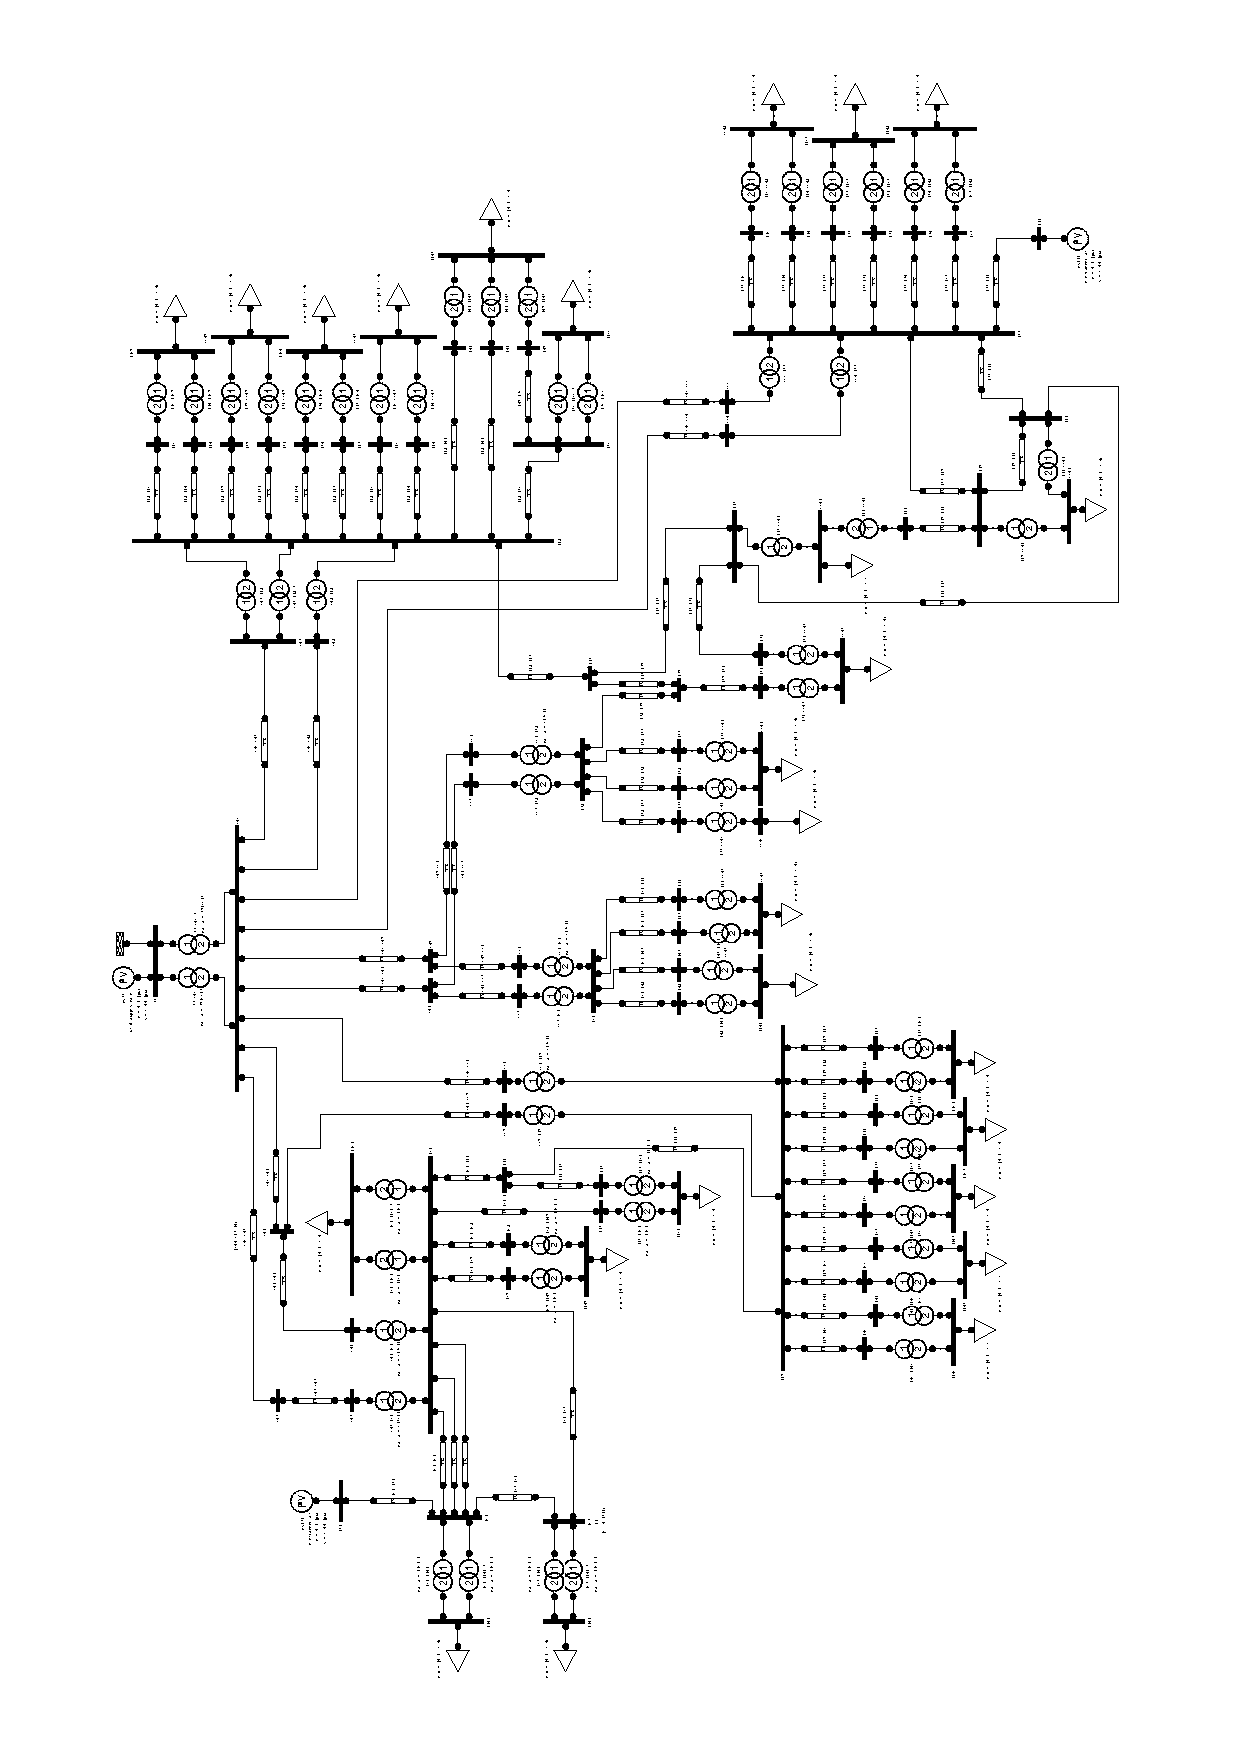
\includegraphics[width=20cm,angle=90]{figures/psat}
  \caption{UKGDS EHV3 model in PSAT Simulink network editor.}
  \label{fig:ukgds_ehv3}
\end{figure}

Optimal power flow problems are solved via an interface to the General
Algebraic Modeling System (GAMS).  GAMS defines optimisation
problems using a high-level modelling language and has a large solver portfolio, including all
of the major commercial and academic solvers.  The interface can be used for
solving single period optimal power flow problems where the objective function
can model maximisation of social benefit, maximisation of the distance to
the maximum loading condition or multi-objective of a combination of these.
Multi-period optimal power flow is formulated as a mixed integer problem with
linearised power balance constraints.  The objective function models
maximisation of social welfare, but is extended to include startup and
shutdown costs.

Power flow and dynamic data are typically separated in electric power
simulation tools, but in PSAT they are integrated.  This combined with the
large number of routines supported by PSAT can make the code base difficult to
understand and modify.  However, comprehensive documentation is included with
PSAT and the mailing list is highly active.  The majority of correspondance on
this list concerns PSAT's dynamic simulation features.  The price of GAMS
licenses and the need for optimal power flow problems to be converted to the
GAMS language before being solved could be considered barriers to its
selection for certain projects.

\subsection*{UWPFLOW}
% Continuation and Direct Methods to Locate Fold Bifurcations in AC/DC/FACTS
% Power Systems
UWPFLOW is a research tool for voltage stability analysis developed at the
University of Waterloo, Ontario, and the University of Wisconsin-Madison.  It
is written in ANSI-C and is available as open source for research purposes
only. The program can be run with the terminal command
\begin{center}
\begin{verbatim}
$ uwpflow [-options] input_file
\end{verbatim}
\end{center}
where \texttt{input\_file} is the path to a data file in the IEEE common data
format (CDF) \cite{cdf:73} that may contain High-Voltage Direct Current (HVDC)
and Flexible Alternating Current Transmission System (FACTS) device data.
Output is also in CDF and can include additional data for post-processing,
including values for nose curve plots.  An interface to UWPFLOW is provided
with PSAT and can be used for bifurcation analysis.

\subsection*{TEFTS}
% Transient Stability Program to Study Energy Functions and Voltage Stability
% (Bifurcation) Phenomena in AC/DC Power Systems
The University of Waterloo also hosts TEFTS -- a transient stability program
for studying energy functions and voltage stability phenomena in AC/HVDC
dynamic power system models.  It too is written in ANSI-C and is licensed for
research purposes only.  An executable file for DOS is provided and the source
package contains a simple example.

\subsection*{Voltage Stability Toolbox}
The Voltage Stability Toolbox (VST) is a \matlab toolbox, developed at the
Center for Electric Power Engineering at Drexel University in Philidelphia, for
investigating stability and bifurcation issues in power systems.  The source
is available for any purpose providing that the authors are suitably cited.
VST features routines for
\begin{itemize}
  \item power flow,
  \item time domain simulation,
  \item static and dynamic bifurcation analysis,
  \item singularity analysis and
  \item eigenvalue analysis.
\end{itemize}
The feature matrix in Table \ref{tbl:featurematrix} shows the similar
capabilities of VST and PSAT. It was developed around the same time and has
the same goals for educational and research applications.  However it does not
have the same quality of documentation nor such an active community of users
and developers as PSAT.

\subsection*{Distribution System Simulator}
In November 2008, the Open Distribution System Simulator (OpenDSS) was released
by the Electric Power Research Institute (EPRI) as open source.  Development of
OpenDSS began in April 1997 and it has been used extensively in distributed
generation impact assessments.  It is the only open source
program designed for both distribution and transmission system simulation.

OpenDSS supports steady-state analysis in the frequency domain, including power
flow, harmonics and dynamics.  Arbitrary n-phase unbalanced circuit analysis is supported using an object orientated data model.  Circuit elements are defined in Object Pascal
and solutions are found using a linear sparse matrix solver written in C and
C++.  OpenDSS is available under the Berkeley Software Distribution (BSD)
license, which allows use for almost any purpose.  Circuits are defined in
scripts, using a domain specific language, that may be executed through a
graphical user interface or a Common Object Model (COM) interface.  The user
interface also provides circuit data editing, plotting and power flow
visualisation tools.

The power flow solver is fast and can be configured for repeated
studies using daily, yearly or duty-cycle data.  The multi-phase circuit model allows
complex fault conditions to be defined and three short-circuit analysis methods
are provided.  The heritage of OpenDSS is in harmonics and dynamics analysis
and it does not support system optimisation.

\subsection*{Agent-based Modelling of Electricity Systems}
\label{sec:ames}
The AMES (Agent-based Modeling of Electricity Systems) power market test bed is
a software package that models core features of the Wholesale Power Market
Platform -- a market design proposed by the Federal Energy Regulatory
Commission (FERC) in April 2003 for common adoption in regions of the
U.S.~\cite{tesfatsi:wpmp}. The market design features:
\begin{itemize}
  \item a centralised structure managed by an independent market operator,
  \item parallel day-ahead and real-time markets and
  \item locational marginal pricing.
\end{itemize}
Learning agents represent load serving entities or generating companies and
learn using Roth-Erev methods (described in Appendix \ref{sec:rotherev})
implemented with the Repast agent simulation toolkit \cite{gieseler:thesis}.
% The permissive license under which the source code for
% these algorithms has been released allowed direct translation of them for use
% in this study.
Agents learn from the solutions of hourly bid/offer based
DC-OPF problems formulated as quadratic programs using the DCOPFJ package
\cite{tesfatsi:dcopf} described in Section \ref{sec:dcopfj}, below.

The capabilities of AMES are demonstrated using a 5-bus network model in
\cite{tesfatsi:pes09}.  The model is provided with AMES and a step-by-step
tutorial describes how it may be used.  AMES comes with a
Swing-based graphical user interface with plotting and table editor tools and
is released under the the \textsc{Gnu} GPL version 2.

\subsection*{DCOPFJ}
\label{sec:dcopfj}
To solve market problems defined in AMES, researchers at Iowa State University
developed a stand-alone DC optimal power flow solver in Java named DCOPFJ.
It formulates optimal power flow problems as convex quadratic programs and
which are solved using QuadProgJ.  The same researcher developed QuadProgJ as
an independant solver that uses the dual active set strictly convex quadratic
programming algorithm \cite{goldfarb:scqp}.  DCOPFJ requires
generator costs to be modelled as polynomial functions, of second order or
less and no sparse matrix techniques are employed to allow application to large
systems.

%\subsection{PyBrain}

\section{Summary}
